\section{Results}

\label{subseq:model estimation}
All the models are estimated to fit the data. In this section there are many parameters which need to be described. The parameters all have their own notation. This means that in the following graphs the following means: $\sigma_{\eta}^2$ is the parameter corresponding to the variance of the state vector, $\sigma_{\epsilon}^2$ is the parameter corresponding to the estimated variance of the error terms, $\beta_1$ corresponds to the first lag of the data, $\beta_7$ corresponds to the seventh lag of the data, $\gamma_1$ corresponds to the weather temperature data, $\gamma_2$ corresponds is the UV index data, $\gamma_3$ corresponds to the number of deliveries, $\gamma_4$ corresponds to the number of regions with vacation, $\gamma_5$ corresponds to 1 if there is a national holiday, 0 otherwise, $\gamma_{6-12}$  are constants for the day of the week and $\theta_0$ is the moving average component. All the graphs of the models can be found in \autoref{sec:forecast results} and the plots of the residuals for all the plots can be found in \autoref{sec:residuals}.\\

\subsection{Forecast results}
\begin{figure}
\begin{minipage}{.5\textwidth}
  \centering
  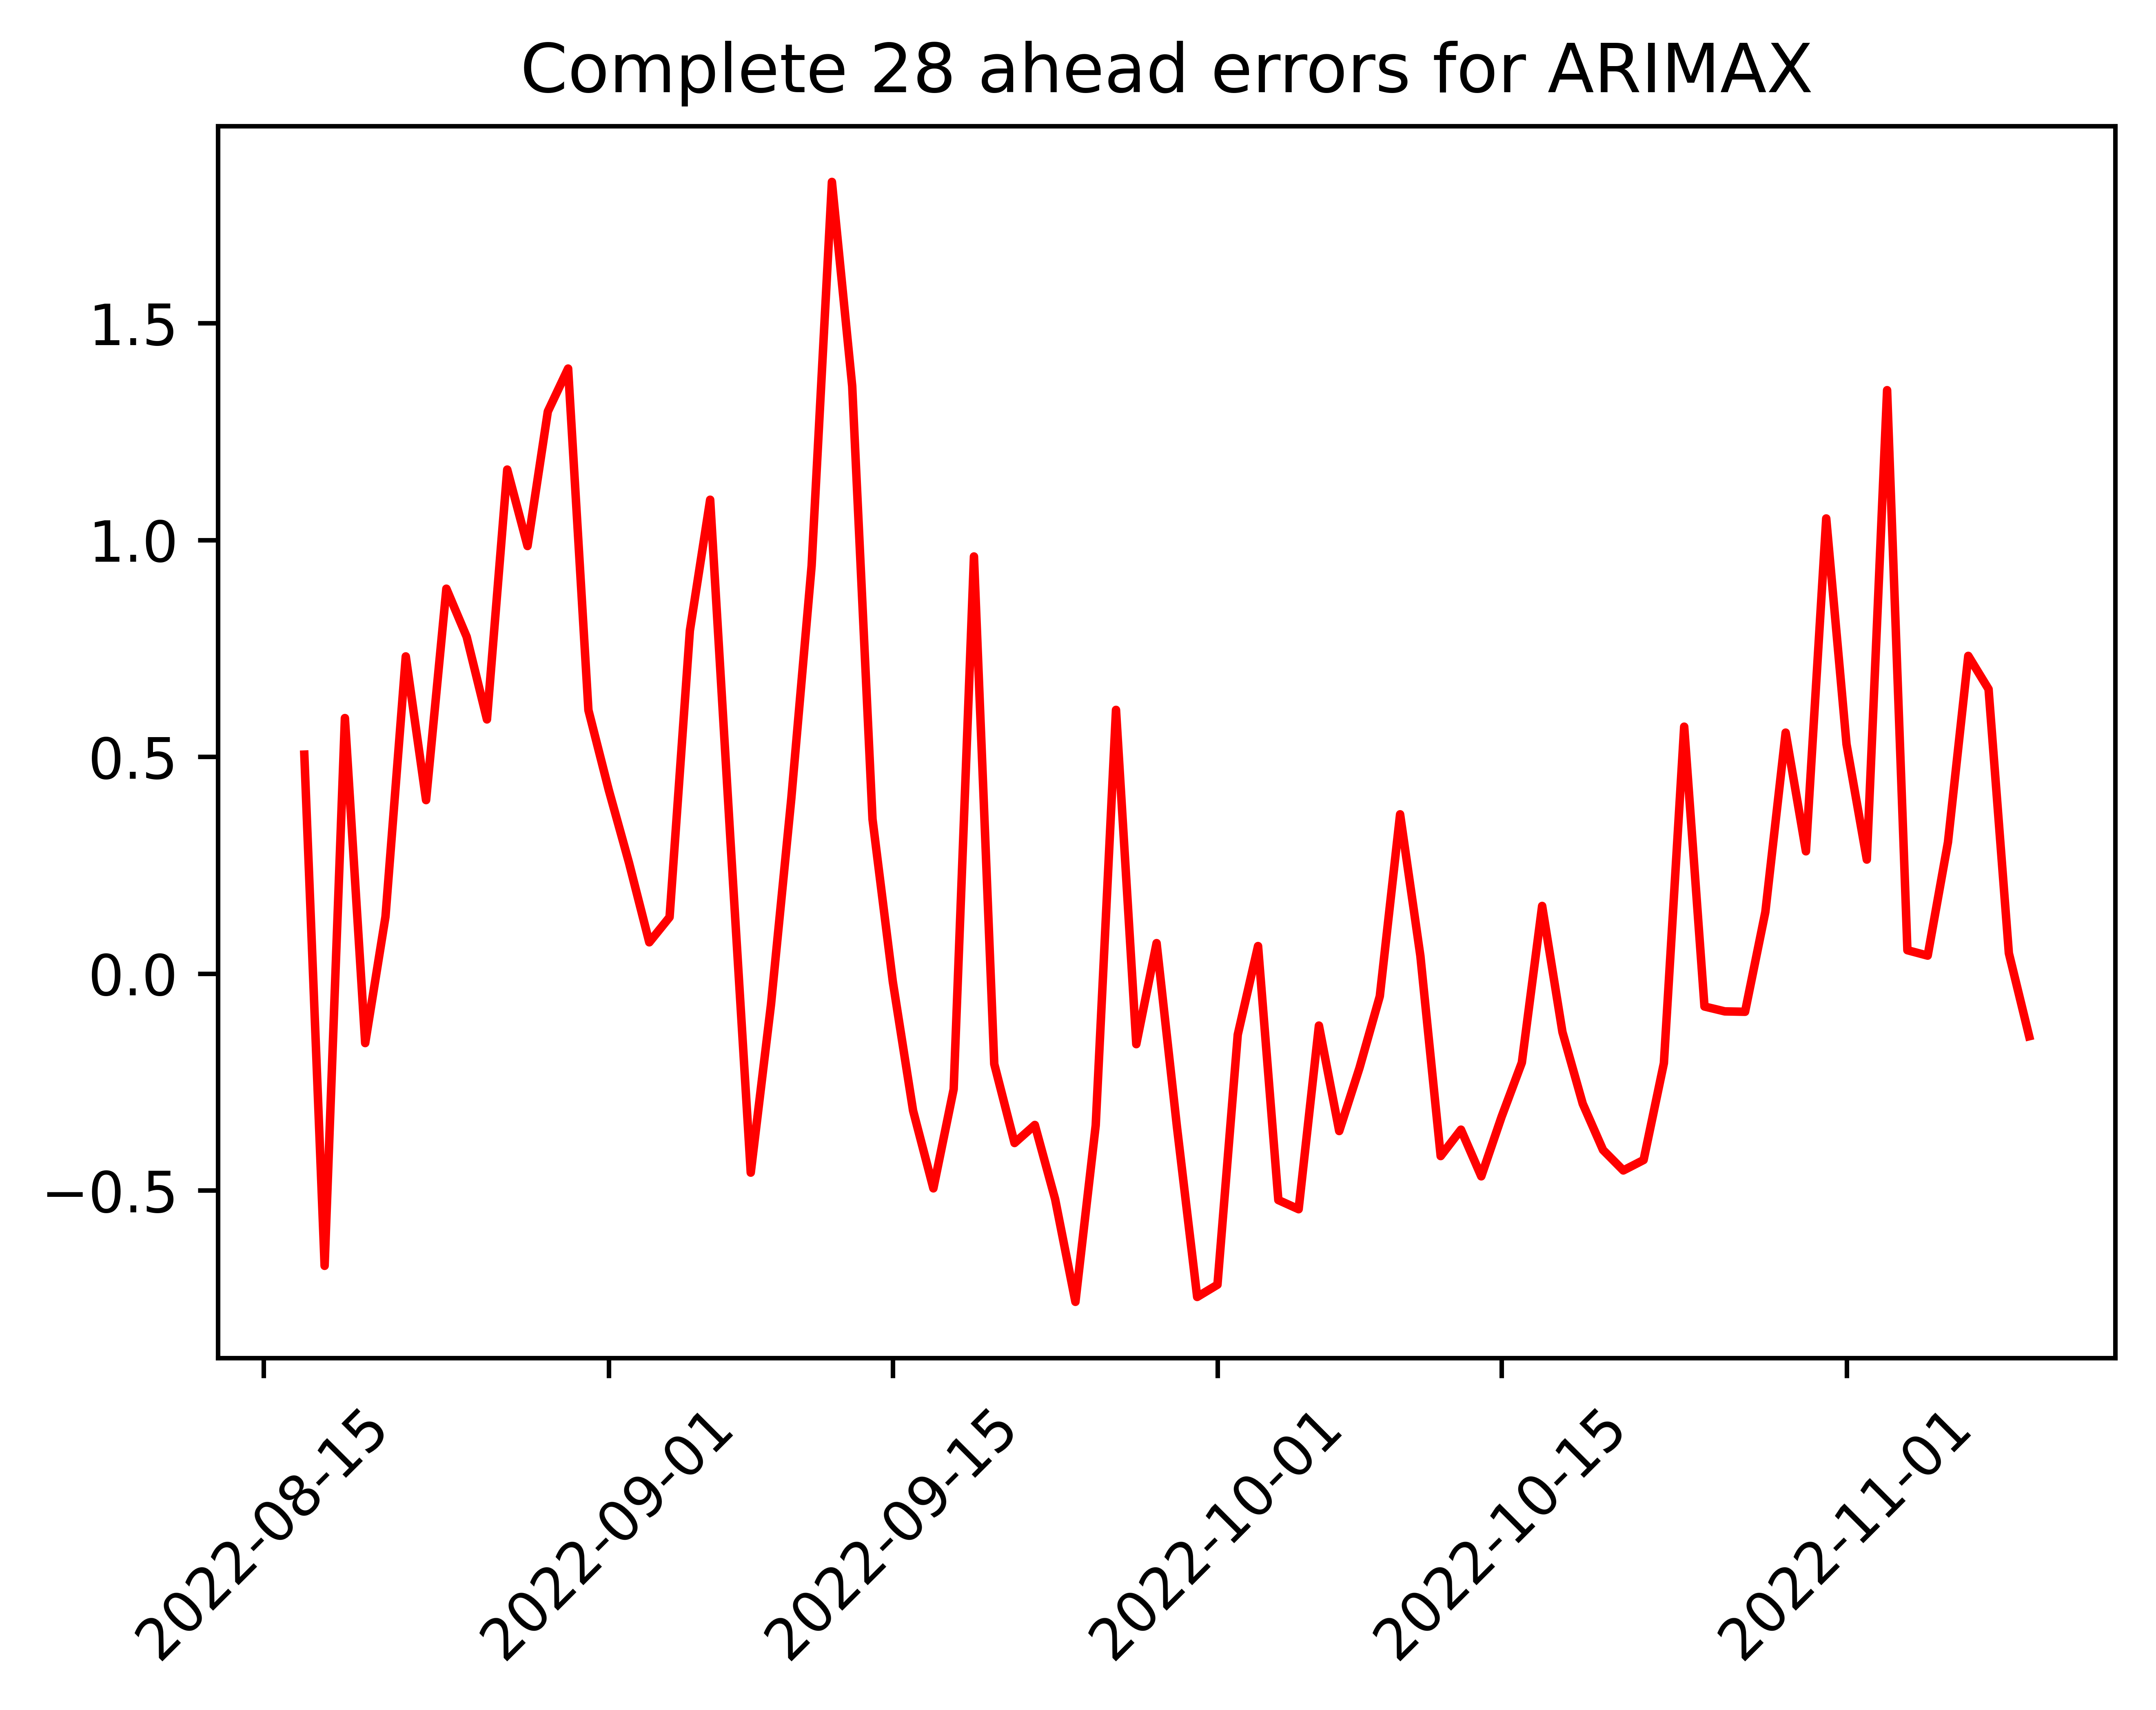
\includegraphics[width=\linewidth]{pics/28_ah/28_ahead_errors_ARIMAX.png}
  \caption{The residuals for the ARIMAX model in the Netherlands}
  \label{fig:ARIMAX 28 ahead}
\end{minipage}
\begin{minipage}{.5\textwidth}
  \centering
  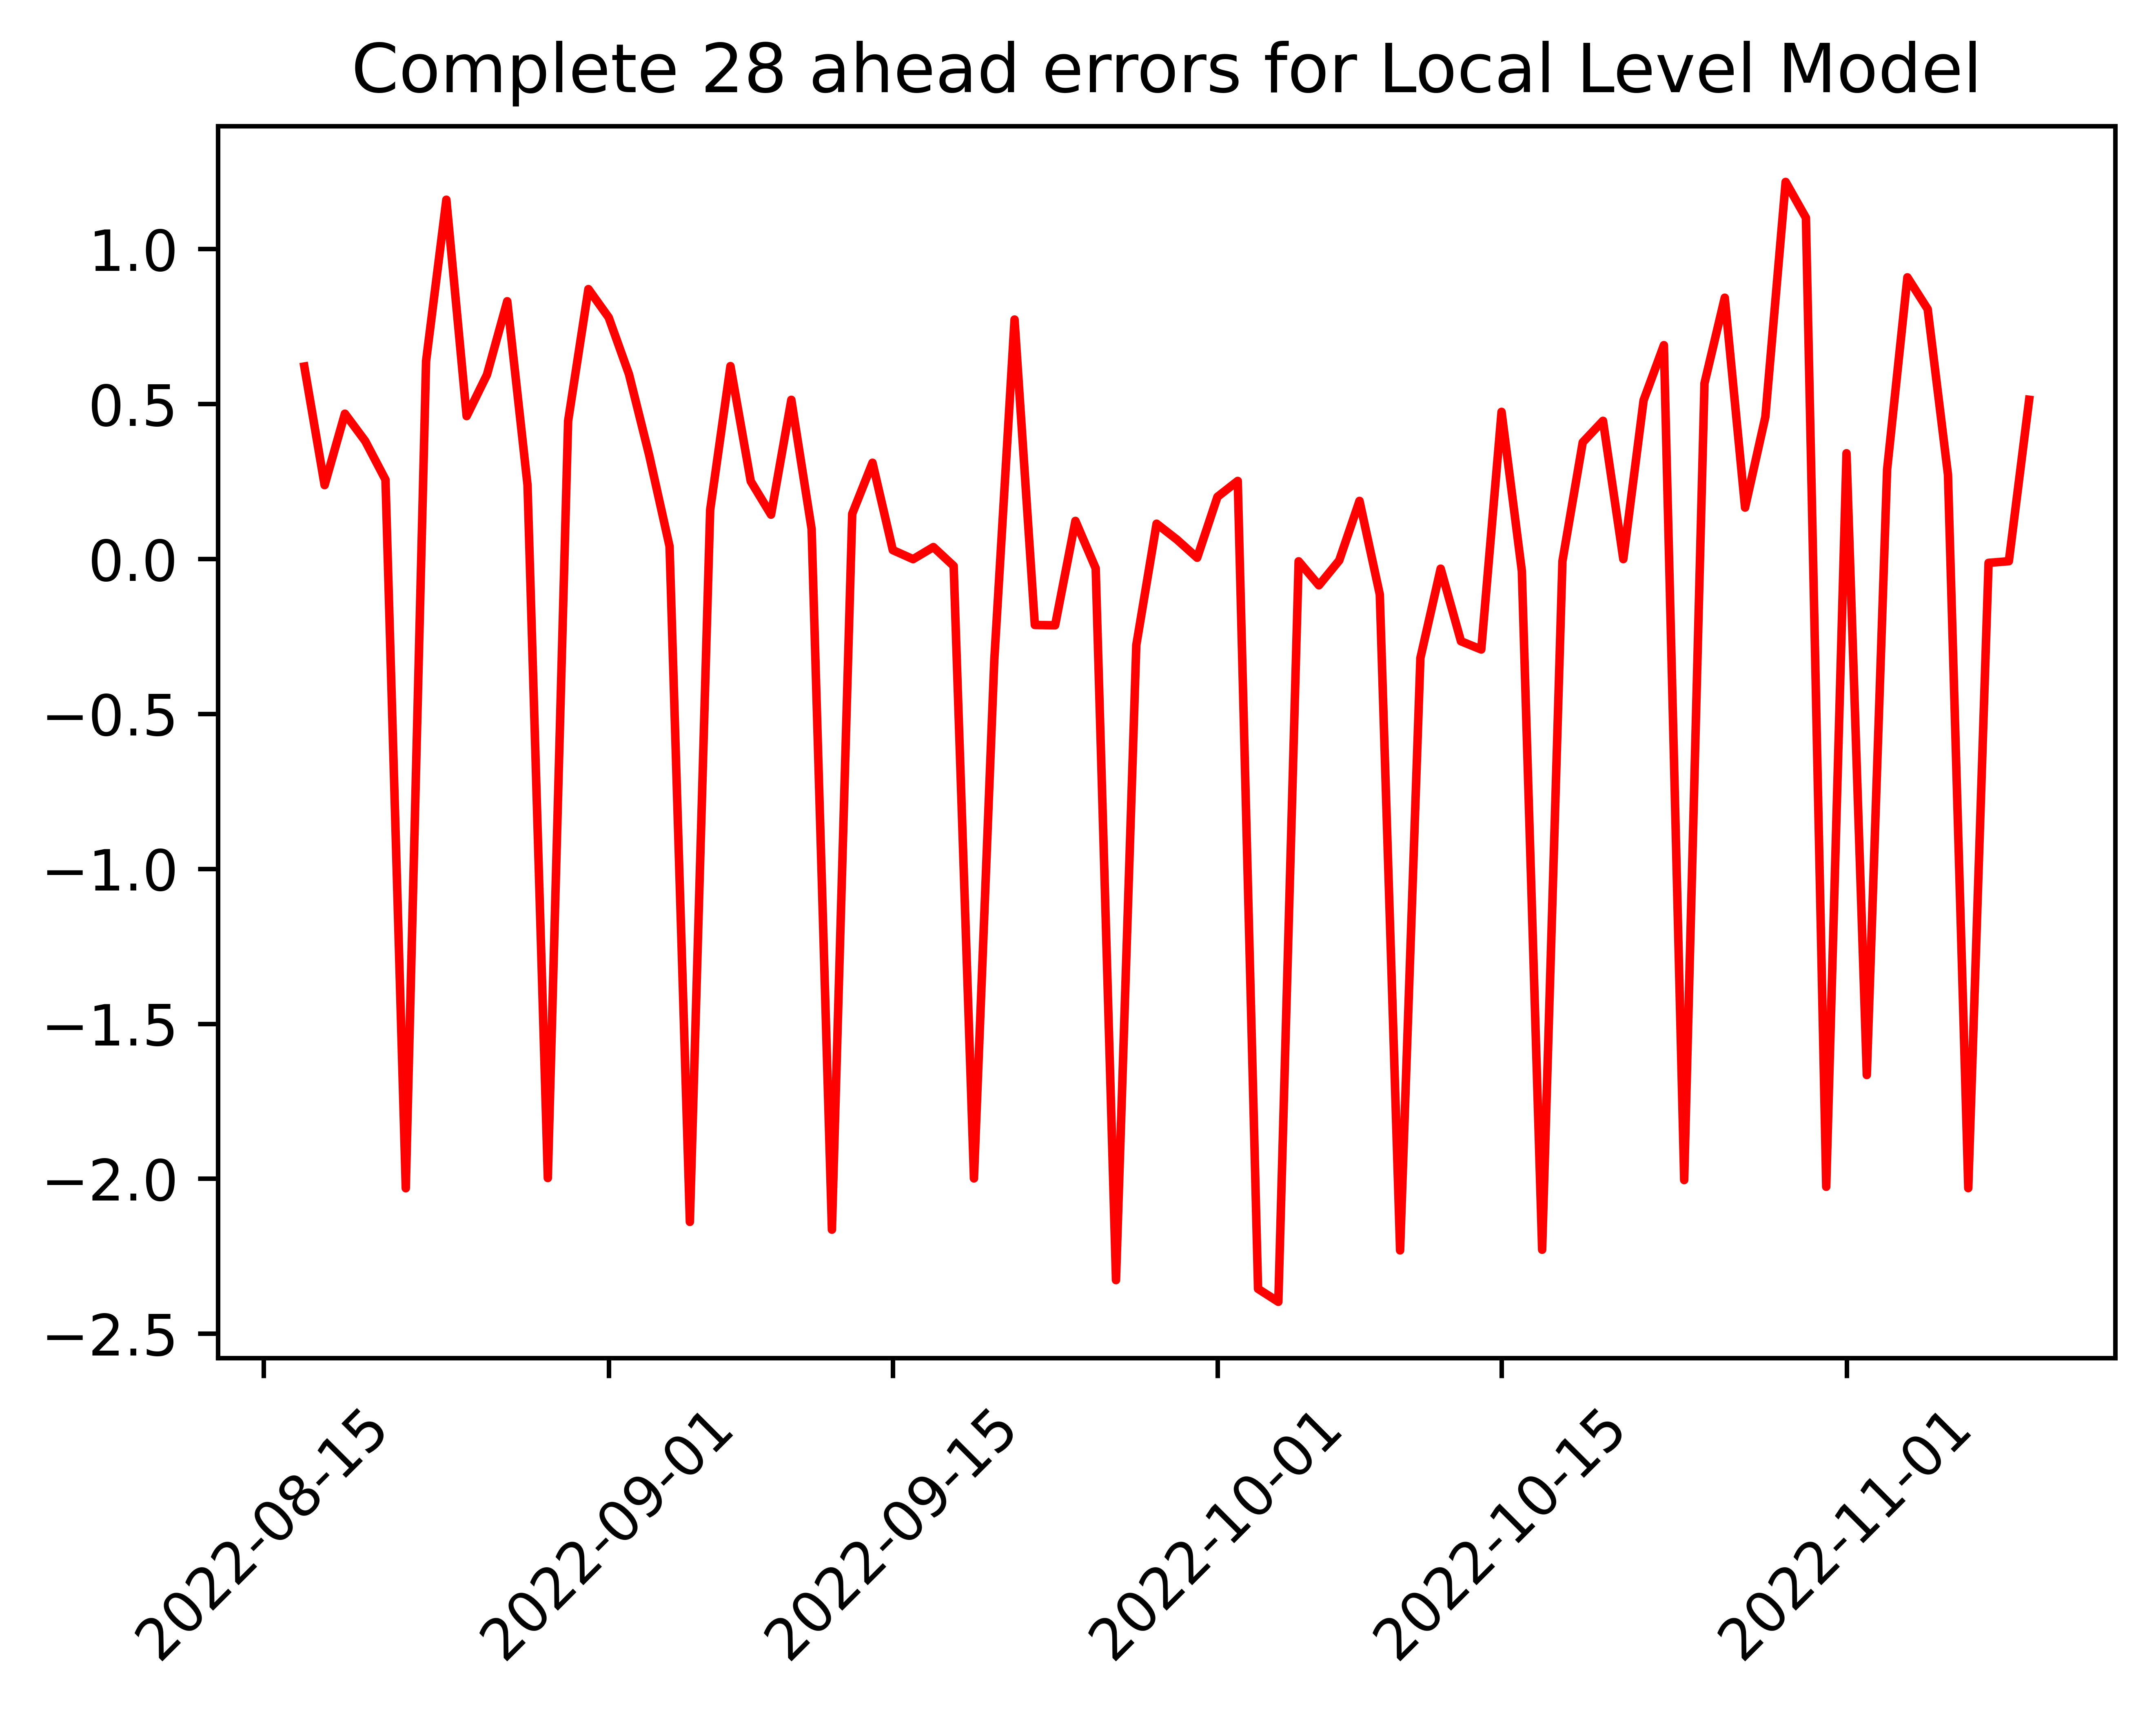
\includegraphics[width=\linewidth]{pics/28_ah/DE_28_ahead_errors_Local Level Model.png}
  \caption{The residuals for the regression model in Germany}
  \label{fig:DE residuals LLM}
\end{minipage}
\end{figure}

\label{subsec:forecast_results}
\begin{table}[]
    \centering
    \begin{tabular}{|c|c c c||c|c c c|}\hline
        NL & coefficient & t-statistic & p-value & DE & coefficient & t-statistic & p-value\\\hline        
        $\sigma_{\epsilon}$ & 0.429 & 10.984 & 0.0 & $\sigma_{\epsilon}$ & 0.349 & 8.943 & 0.0\\
        $\sigma_{\eta}$ & 0.002 & 0.044 & 0.965 & $\sigma_{\eta}$ & 0.001 & 0.015 & 0.988\\\hline
    \end{tabular}
    \caption{Local level model regression results with the coefficient, t-statistic and p-values for the Dutch and German estimation}
    \label{tab:local_level_regression_Results}
\end{table}
The most basic model is the local level model with two estimated values of $\sigma$. The estimated parameters of this model can be found in \autoref{tab:local_level_regression_Results}. The value of $\sigma_{\epsilon}$ is quite large and therefore also significant for both the Dutch and the German data with a p-value smaller than 0.0005. This makes a very low signal to noise ratio of 0.0047 for the Netherlands and 0.0029 for Germany. That means there is there is a lot of noise in the data which is expected as cases at customer service can come with a very high variance. The estimated values of $\sigma_{\eta}$  is in both cases much smaller and definitely not significant.\\

\begin{table}[]
    \centering
    \begin{tabular}{|c|c c c||c|c c c|}\hline
        NL & coefficient & t-statistic & p-value & DE & coefficient & t-statistic & p-value\\\hline     
        $\sigma_{\epsilon}$ & 0.236 & 6.046 & 0.0 & $\sigma_{\epsilon}$ & 0.031 & 0.791 & 0.429\\
        $\sigma_{\eta}$ & 0.001 & 0.013 & 0.99 & $\sigma_{\eta}$ & 0.002 & 0.05 & 0.96\\
        $\gamma_{1}$ & 0.033 & 0.828 & 0.408 & $\gamma_{1}$ & 0.068 & 1.686 & 0.092\\
        $\gamma_{2}$ & 0.048 & 1.231 & 0.219 & $\gamma_{2}$ & 0.035 & 0.887 & 0.375\\
        $\gamma_{3}$ & 0.268 & 8.194 & 0.0 & $\gamma_{3}$ & 0.856 & 25.361 & 0.0\\
        $\gamma_{4}$ & -0.15 & -3.935 & 0.0 & $\gamma_{4}$ & -0.015 & -0.413 & 0.68\\
        $\gamma_{5}$ & -0.163 & -4.37 & 0.0 & $\gamma_{5}$ & -0.038 & -0.957 & 0.339\\
        $\gamma_{6}$ & 0.557 & 15.406 & 0.0 & $\gamma_{6}$ & 0.306 & 8.883 & 0.0\\
        $\gamma_{7}$ & 0.284 & 8.299 & 0.0 & $\gamma_{7}$ & 0.34 & 10.032 & 0.0\\
        $\gamma_{8}$ & 0.349 & 9.812 & 0.0 & $\gamma_{8}$ & 0.369 & 10.401 & 0.0\\
        $\gamma_{9}$ & 0.298 & 7.631 & 0.0 & $\gamma_{9}$ & 0.365 & 9.439 & 0.0\\
        $\gamma_{10}$ & 0.489 & 15.576 & 0.0 & $\gamma_{10}$ & 0.359 & 11.397 & 0.0\\
        $\gamma_{11}$ & 0.306 & 8.935 & 0.0 & $\gamma_{11}$ & 0.307 & 9.586 & 0.0\\
        $\gamma_{12}$ & 0.16 & 4.737 & 0.0 & $\gamma_{12}$ & 0.245 & 7.53 & 0.0\\\hline
    \end{tabular}
    \caption{Regression model results with the coefficient, t-statistic and p-values for the Dutch and German estimation}
    \label{tab:regression_model_results}
\end{table}
The expansion of the local level model to the regression model with parameters to the regression model described in \autoref{tab:regression_model_results}. The regression model only has a significant $\sigma_{\epsilon}$ in the Dutch data. The German data has no significant $\sigma_\epsilon$. This is probably because the German data has more steep differences in the data which can be explained better by other factors like the day of the week. Just as with the local level model, the $\sigma_\eta$ is in both countries not significant. Something to note is that the weather data ($\gamma_1$ and $\gamma_2$) are not significant in the Netherlands with parameters of only 0.268 and -0.15, but the temperature ($\gamma_2$) in Germany is significant at the 10\% significance interval with a coefficient of 0.375. The number of deliveries ($\gamma_3$) is significant in both the Netherlands and Germany and it is worth it to take a look at how large the difference is between the Netherlands (0.268) and Germany (0.856) in Number of deliveries coefficient pointing to a more reliable cases per delivery relationship in Germany. The coefficients corresponding to vacations ($\gamma_4$) and holidays ($\gamma_5$) are significant in the Netherlands and not in Germany. This could be because the German operations have more days where the Customer Service is offline and there are no deliveries. In the Netherlands this only happens at holidays, but in Germany this happens also at Sundays. In the plot of the residuals in Germany in \autoref{fig:DE residuals LLM} you can clearly see there are large negative residuals at every Sunday for the local level model. The last thing to point out is that all the constants for the different days ($\gamma_6$-$\gamma_{12}$) are significant, pointing to a strong relation between what day it is and how many cases come in.\\

\begin{table}[]
    \centering
    \begin{tabular}{|c|c c c||c|c c c|}\hline
        NL & Coefficient & t-statistic & p-value & DE & Coefficient & t-statistic & p-value\\\hline
        $\beta_1$ & 0.154 & 3.867 & 0.0 & $\beta_1$ & 0.177 & 4.594 & 0.0\\
        $\beta_7$ & 0.500 & 12.598 & 0.0 & $\beta_7$ & 0.814 & 21.104 & 0.0\\
        $\theta_0$ & -0.043 & -1.112 & 0.267 & $\theta_0$ & -0.045 & -1.147 & 0.252\\\hline
    \end{tabular}
    \caption{ARIMA regression results with the coefficient, t-statistic and p-values for the Dutch and German estimation}
    \label{tab:ARIMA_estimation_results}
\end{table}
In the results of the ARIMA regression are given in in \autoref{tab:ARIMA_estimation_results}. It is remarkable that the moving average components are not significant for both countries. Also note that the seventh lag ($\beta_7$) has a higher coefficient than the first lag, pointing to a strong weekly relationship.\\

\begin{table}[]
    \centering
    \begin{tabular}{|c|c c c||c|c c c|}\hline
        NL & Coefficient & t-statistic & p-value & DE & Coefficient & t-statistic & p-value\\\hline
        $\gamma_{1}$ & 0.04 & 1.011 & 0.312 & $\gamma_{1}$ & 0.086 & 2.17 & 0.03\\
        $\gamma_{2}$ & 0.04 & 0.997 & 0.319 & $\gamma_{2}$ & 0.052 & 1.293 & 0.196\\
        $\gamma_{3}$ & 0.334 & 8.372 & 0.0 & $\gamma_{3}$ & 0.800 & 22.371 & 0.0\\
        $\gamma_{4}$ & -0.089 & -2.301 & 0.022 & $\gamma_{4}$ & 0.002 & 0.047 & 0.963\\
        $\gamma_{5}$ & -0.128 & -3.006 & 0.003 & $\gamma_{5}$ & -0.041 & -0.977 & 0.329\\
        $\gamma_{6}$ & 0.151 & 3.857 & 0.0 & $\gamma_{6}$ & 0.174 & 4.434 & 0.0\\
        $\gamma_{7}$ & -0.155 & -3.948 & 0.0 & $\gamma_{7}$ & 0.098 & 2.503 & 0.013\\
        $\gamma_{8}$ & -0.022 & -0.565 & 0.572 & $\gamma_{8}$ & 0.106 & 2.703 & 0.007\\
        $\gamma_{9}$ & -0.077 & -1.964 & 0.05 & $\gamma_{9}$ & 0.106 & 2.725 & 0.007\\
        $\gamma_{10}$ & 0.06 & 1.547 & 0.122 & $\gamma_{10}$ & 0.097 & 2.483 & 0.013\\
        $\gamma_{11}$ & -0.139 & -3.566 & 0.0 & $\gamma_{11}$ & 0.033 & 0.849 & 0.396\\
        $\gamma_{12}$ & -0.176 & -4.517 & 0.0 & $\gamma_{12}$ & 0.005 & 0.14 & 0.889\\
        $\beta_{1}$ & 0.206 & 5.176 & 0.0 &$\beta_{1}$ & 0.186 & 4.823 & 0.0\\
        $\beta_{7}$ & 0.131 & 3.287 & 0.001 & $\beta_{7}$ & 0.063 & 1.628 & 0.104\\
        $\theta_{0}$ & 0.049 & 1.281 & 0.201 & $\theta_0$ & 0.229 & 21.508 & 0.0\\\hline
    \end{tabular}
    \caption{ARIMAX regression results with the coefficient, t-statistic and p-values for the Dutch and German estimation}
    \label{tab:arimax_estimation}
\end{table}
The estimated parameters of the ARIMAX regression are given in \autoref{tab:arimax_estimation} and tell us more about the interaction between the explanatory variables and the lags. Just as in the regression model, the weather data only has a significant effect on the German cases and from the two weather variables, only the temperature ($\gamma_1$) has a significant effect with a coefficient of 0.086. Also as in the regression model, the number of deliveries ($\gamma_3$) has a strong effect on both data sets, but it has an even larger effect in the German data with coefficients of 0.800 in Germany against only 0.344. Things start to become different looking at the national holidays ($\gamma_6$) which is significant in the ARIMAX model for Germany, but not in the regression model. The coefficient corresponding to the national holidays is 0.151 in the Netherlands and 0.174 in Germany which is a large difference with the regression model. Another important difference between the ARIMAX model and the regression model is that the daily constants have a very different level of significance. The regressors are smaller and multiple daily constants have no significance at the 5\% significance level. A remarkable result is the non significance of the Sunday constant $\lambda_{12}$ in Germany which has has coefficient of only 0.063. The German Sunday drop in cases is not explained as a drop in cases on Sunday by the ARIMAX model, but with the drop in deliveries at Sundays. You can also see a difference with the ARIMA as we see the seventh lag drop in importance and in the German data, the seventh lag is not even significant at the 10\% significance level. Another difference with the ARIMA model is that the German data has a significant moving average component with a coefficient of 0.229 comparing to the Dutch moving average component of 0.049.\\

\begin{table}[]
    \centering
    \begin{tabular}{|c|c c c||c|c c c|}\hline
        NL & Coefficient & t-statistic & p-value & DE & Coefficient & t-statistic & p-value\\\hline
        $\gamma_{1}$ & 0.041 & 1.076 & 0.282 & $\gamma_{1}$ & 0.084 & 2.157 & 0.031\\
        $\gamma_{2}$ & 0.041 & 1.096 & 0.273 & $\gamma_{2}$ & 0.052 & 1.27 & 0.205\\
        $\gamma_{3}$ & 0.338 & 9.636 & 0.0 & $\gamma_{3}$ & 0.795 & 20.94 & 0.0\\
        $\gamma_{4}$ & -0.089 & -2.509 & 0.012 & $\gamma_{4}$ & 0.001 & 0.028 & 0.978\\
        $\gamma_{5}$ & -0.125 & -3.518 & 0.0 & $\gamma_{5}$ & -0.041 & -1.045 & 0.296\\
        $\gamma_{6}$ & 0.22 & 6.54 & 0.0 & $\gamma_{6}$ & 0.066 & 1.96 & 0.05\\
        $\gamma_{7}$ & -0.075 & -2.357 & 0.019 & $\gamma_{7}$ & -0.0 & -0.0 & 1.0\\
        $\gamma_{8}$ & 0.05 & 1.493 & 0.136 & $\gamma_{8}$ & 0.006 & 0.182 & 0.856\\
        $\gamma_{9}$ & 0.0 & 0.0 & 1.0 & $\gamma_{9}$ & 0.006 & 0.153 & 0.879\\
        $\gamma_{10}$ & 0.131 & 4.184 & 0.0 & $\gamma_{10}$ & -0.002 & -0.049 & 0.961\\
        $\gamma_{11}$ & -0.062 & -1.908 & 0.057 & $\gamma_{11}$ & -0.063 & -2.022 & 0.044\\
        $\gamma_{12}$ & -0.098 & -3.117 & 0.002 & $\gamma_{12}$ & -0.085 & -2.73 & 0.007\\
        $\beta_{1}$ & 0.199 & 6.267 & 0.0 & $\beta_{1}$ & 0.174 & 5.803 & 0.0\\
        $\beta_{7}$ & 0.133 & 4.365 & 0.0 & $\beta_{7}$ & 0.078 & 2.587 & 0.01\\
        $\lambda^{(1)}$ & -0.846 & -0.0 & 1.0 & $\lambda^{(1)}$ & -0.811 & -0.0 & 1.0\\
        $\lambda^{(2)}$ & -0.104 & -0.0 & 1.0 & $\lambda^{(2)}$ & -0.104 & -0.0 & 1.0\\ \hline
    \end{tabular}
    \caption{Fused lasso regression results with the coefficient, t-statistic and p-values for the Dutch and German estimation}
    \label{tab:FLASSO_estimation_results}
\end{table}
The fused lasso seems to behave in a way that is very similar to the ARIMAX. This is not really surprising as the regression results given in \autoref{tab:FLASSO_estimation_results} show two insignificant values of $\lambda$, and the values of $\theta_0$ in the ARIMAX model are also insignificant (\autoref{tab:arimax_estimation}). The expectation would be that the coefficients are very close to the ARIMAX coefficients. The exception to this are the day of the week constants. So in line with this it seems like the regressions of the ARIMA and the LASSO are not very much different for the Dutch data which is supported by the Diebold Mariano tests. The regressions however are different from each other with the German data as it has larger coefficients for the weekday variables which are different with the two models.\\


\label{seq:results}
In this section, the fitted parameters of the parametric models will be reported, as well as the performance of each model.
\subsection{Model Estimation}
\begin{figure}
\begin{minipage}{.5\textwidth}
  \centering
  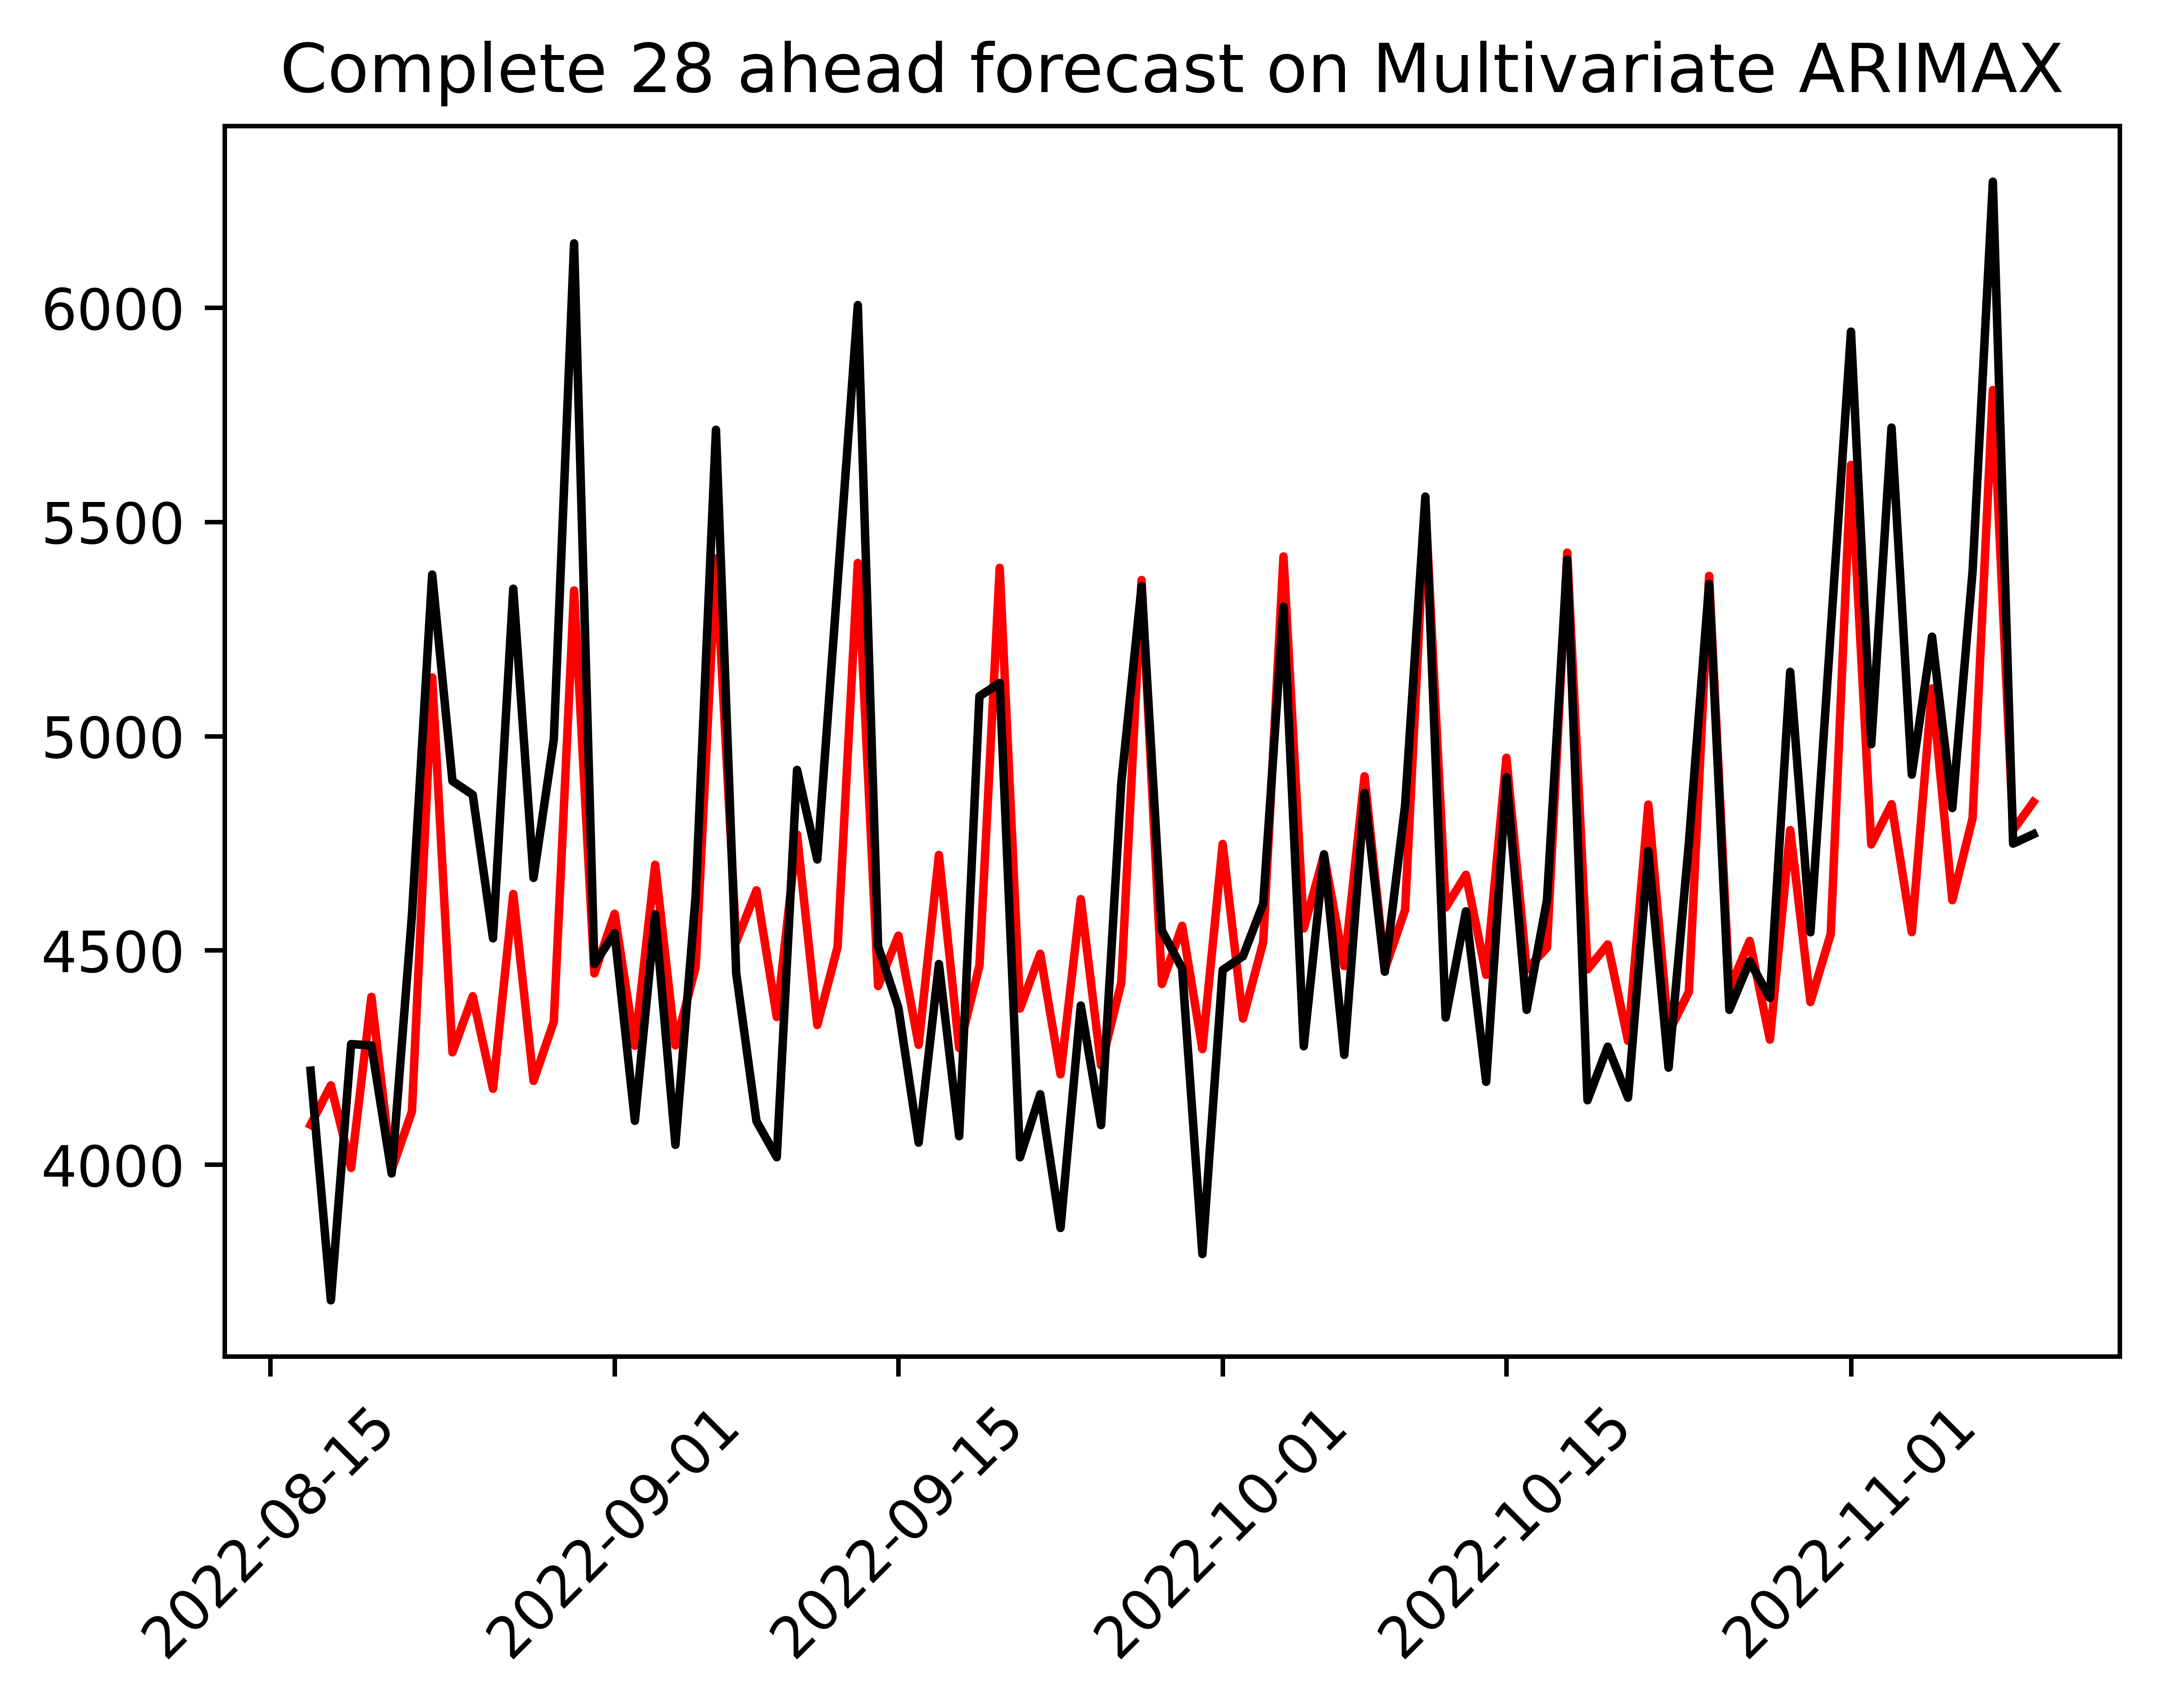
\includegraphics[width=\linewidth]{pics/28_ah/Complete_28_ahead_Multivariate ARIMAX.png}
  \caption{VARIMAX regression (red) and the true values (black) of the total number of cases in the Netherlands}
  \label{fig:ARIMAX 28 ahead}
\end{minipage}
\begin{minipage}{.5\textwidth}
  \centering
  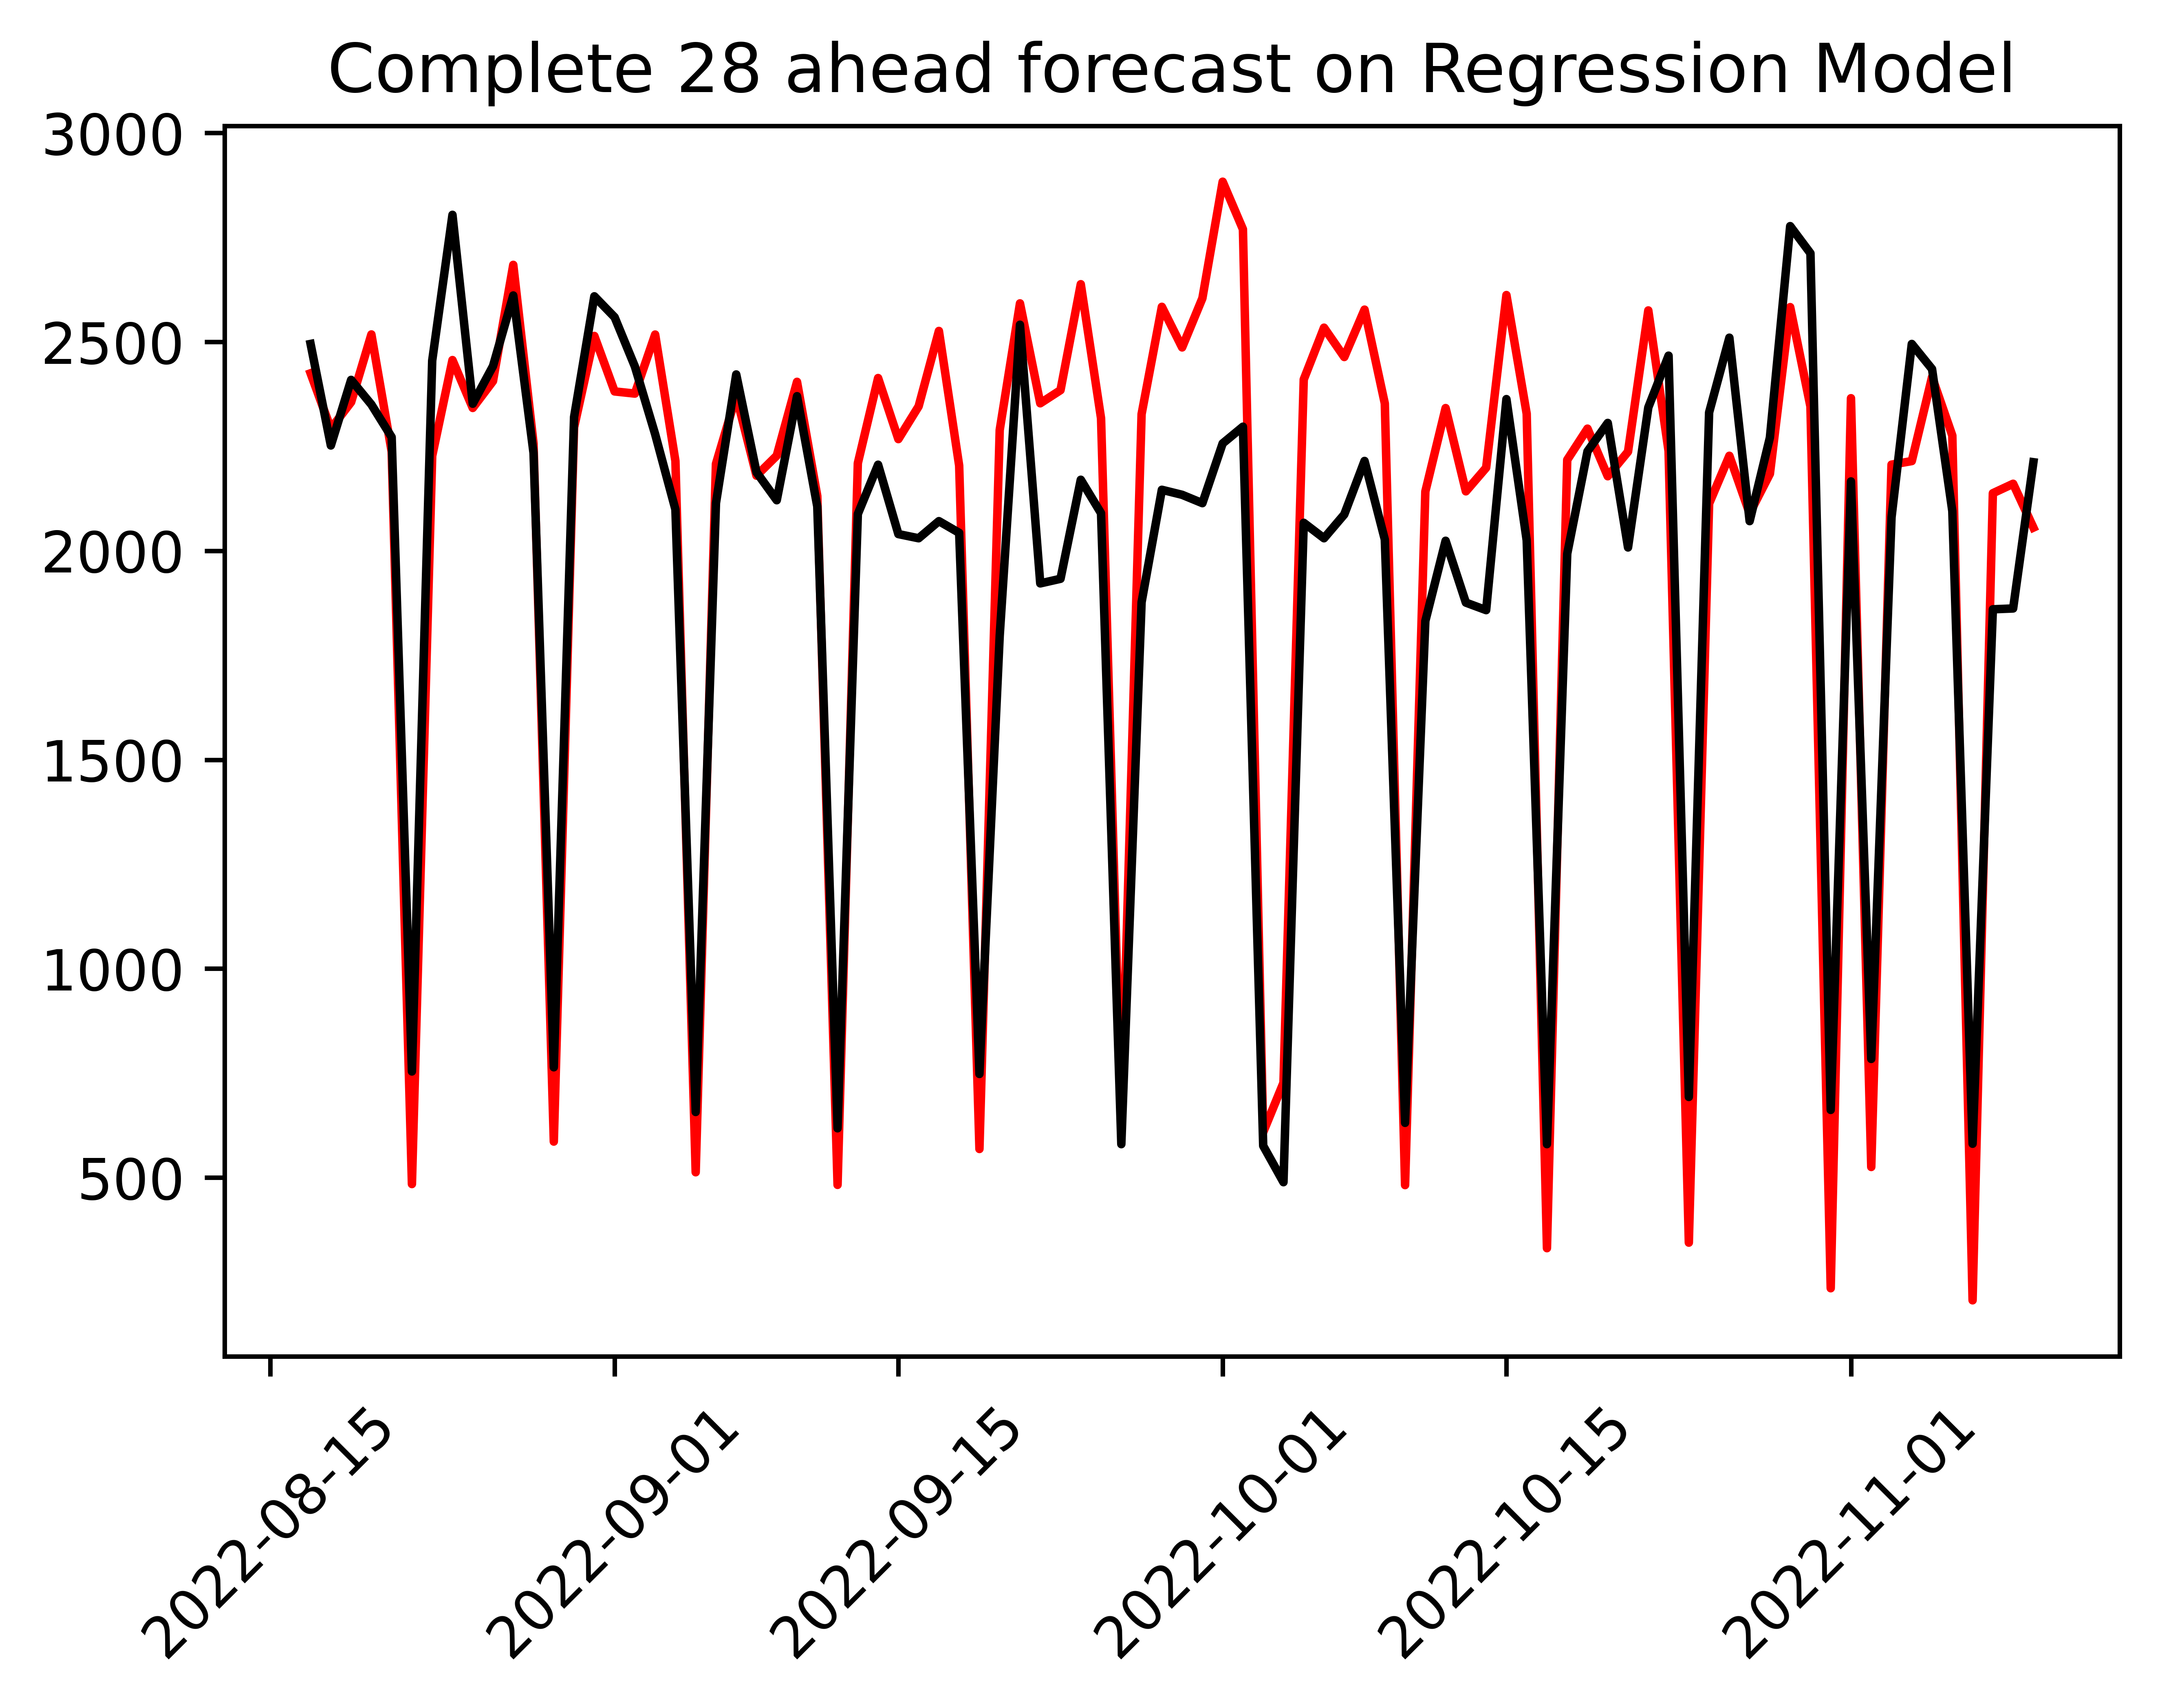
\includegraphics[width=\linewidth]{pics/28_ah/DE_Complete_28_ahead_Regression Model.png}
  \caption{The total number of cases (red) regression and the true values (black) for the regression model in Germany}
  \label{fig:DE regression model}
\end{minipage}
\end{figure}

The performance of the forecasts are measured on the similarity to the test set. There are tests performed on three horizons of forecasts: 7 days (\autoref{tab:1 week ahead}), 28 days (\autoref{tab:4 weeks ahead}) and 49 days (\autoref{tab:7 weeks ahead}). For all the models the MAE (Mean Absolute Error), MSE (Mean Squared Error), RMSE (root Mean Squared Error) and MAPE (Mean Absolute Percentage Error) are calculated. We see that all of the models perform better on the Dutch data. This can be expected because the Dutch operations are going on for a longer and are more mature while the German operations are newer and less mature. The p-values of the Diebold Mariano test can be seen in Tables \ref{tab:1 week ahead diebold}, \ref{tab:4 week ahead dm} and \ref{tab:7 weeks ahead dm} for the 1 week, 4 weeks and 7 weeks horizons.\\

The better performance in the Netherlands can have multiple reasons. The Germans have done good work improving the picking process at the fulfillment centers and streamlining customer communication. This however means that the models cannot yet learn from these improvements as they are continuously implemented. It is possible that as the German market matures the models in the future will improve their performance.\\

\begin{table}[]
    \centering
    \begin{tabular}{|c|c c c|}\hline
        Netherlands & MAE & RMSE & MAPE\\\hline
        Local Level Model & 384.729  & 496.16 & 0.114\\
        Regression Model & 299.849 & 385.391 & 0.087\\
        ARIMA & 286.902 & 412.48 & 0.078\\
        ARIMAX & 242.294 & 322.536 & 0.068\\
        VARIMAX & 250.475 & 325.205 & 0.071\\
        Fused Lasso & 240.894 & 321.319 & 0.068\\
        XGBoost & 308.925 & 418.073 & 0.088\\
        Neural Network & 291.157 & 365.504 & 0.083\\
        Multivariate Neural Network & 311.359 & 390.876 & 0.09\\
        Mixed Model & 266.868 & 342.778 & 0.076\\\hline\hline
        Germany & MAE & RMSE & MAPE\\\hline
        Local Level Model & 435.601 & 631.483 & 0.223\\
        Regression Model & 198.15 & 237.948 & 0.238\\
        ARIMA & 261.571 & 393.473 & 0.191\\
        ARIMAX & 280.529 & 328.543 & 0.16\\
        VARIMAX & 277.817 & 328.396 & 0.152\\
        Fused Lasso & 275.518 & 323.531 & 0.157\\
        XGBoost & 292.353 & 356.378 & 0.186\\
        Neural Network & 302.738 & 356.812 & 0.179\\
        Multivariate Neural Network & 352.059 & 409.035 & 0.199\\
        Mixed Model & 301.783 & 359.547 & 0.175\\\hline  
    \end{tabular}
    \caption{Quality Measures mean absolute error (MAE), root mean squared error (RMSE) and the mean absolute percentage error (MAPE) for the different models types on the 7 steps ahead forecast (1 week) for test data on the total number of cases given in \autoref{fig:total cases NL} \& \ref{fig:total cases DE}}
    \label{tab:1 week ahead}
\end{table}

\begin{table}[]
    \centering
    \begin{tabular}{|c|c c c|}\hline
        Netherlands & MAE & RMSE & MAPE\\\hline
        Local Level Model & 445.285 & 588.893 & 0.134\\
        Regression Model & 329.781 & 432.864 & 0.097\\
        ARIMA & 420.877 & 582.441 & 0.108\\
        ARIMAX & 250.301 & 349.449 & 0.067\\
        VARIMAX & 251.796 & 341.498 & 0.068\\
        Fused Lasso & 249.305 & 348.53 & 0.067\\
        XGBoost & 334.567 & 434.145 & 0.092\\
        Neural Network & 311.201 & 382.848 & 0.088\\
        Multivariate Neural Network & 494.833 & 633.21 & 0.104\\
        Mixed Model & 266.449 & 348.092 & 0.074\\\hline\hline
        Germany & MAE & RMSE & MAPE\\\hline
        Local Level Model & 436.449 & 622.384 & 0.223\\
        Regression Model & 230.472 & 252.553 & 0.289\\
        ARIMA & 484.311 & 557.738 & 0.3\\
        ARIMAX & 289.167 & 343.674 & 0.155\\
        VARIMAX & 281.7 & 339.411 & 0.145\\
        Fused Lasso & 287.661 & 342.398 & 0.154\\
        XGBoost & 304.611 & 365.341 & 0.192\\
        Neural Network & 326.643 & 389.907 & 0.184\\
        Multivariate Neural Network & 418.576 & 485.37 & 0.223\\
        Mixed Model & 321.108 & 388.812 & 0.177\\\hline
    \end{tabular}
    \caption{ Quality Measures mean absolute error (MAE), root mean squared error (RMSE) and the mean absolute percentage error (MAPE) for the different models types on the 28 steps ahead forecast (4 weeks) in the Netherlands and Germany for test data on the total number of cases given in \autoref{fig:total cases NL} \& \ref{fig:total cases DE} }
    \label{tab:4 weeks ahead}
\end{table}

The local level model did not show the best performance but serves as a good basis level. The model does not find patterns in the data as other methods do, but is more an estimation of the mean of the data. This can be a good estimate but in the case of these two data sets for Customer Service it does not perform very well with an RMSE that is in most cases between 400 and 450.\\

The regression model performed better than what we expected, especially in Germany. In the Netherlands, it was not significantly better than the fused Lasso and ARIMAX forecasts on the 7 and 28 steps horizons. In Germany the regression model did even better, outperforming all the other models by the RMSE and MAE, but as noted in \autoref{subsec:forecast_results}, the MAPE suffers from some low predicted values, making the denominator very small. The 28 ahead forecast results are plotted in \autoref{fig:DE regression model}.\\

The ARIMA model had a moderate performance in the Netherlands but performed under our expectations. An explanation for this could be that the data has a larger correlation with the explanatory data than with the lags alone. This is also supported by the good performance of the regression model. The difference in performance is even larger in Germany with an RMSE of 393 (\autoref{tab:1 week ahead}), 557 (\autoref{tab:4 weeks ahead}) and 674 (\autoref{tab:7 weeks ahead}). The worse performance in Germany is to some extent expected as the ARIMA model does not have any parameter that can compensate for the large variance on Sundays in Germany. In the Netherlands, the ARIMA model was not significantly different that the local Level Model, while in Germany the ARIMA model was even worse than the local level model.\\

The ARIMAX model performed better than the ARIMA and local level model, but did not outperform the regression model on every horizon in the Netherlands. The ARIMAX model has a performance very similar to the performance of the fused Lasso. The difference between the ARIMAX forecast and the Fused Lasso forecast is not significant for both the Dutch and the German data (Tables \ref{tab:1 week ahead diebold}, \ref{tab:4 week ahead dm} \& \ref{tab:7 weeks ahead dm}). Overall, the ARIMAX model had the best performance at some metrics of the univariate models in the Netherlands, but was always tied with the fused Lasso model. The ARIMAX was able to take advantage in the data patterns of the explanatory data and the lagged dependent data both.\\

The VARIMAX model had a great performance, outperforming all the other models in the longer horizons in the Netherlands and still creating a reasonable performance in Germany. The 28 ahead forecast for the test data in the Netherlands in plotted in \autoref{fig:ARIMAX 28 ahead} In Germany only the regression Model managed to get a better performance on the MAE and RMSE. A disadvantage of this model might be that it is computationally heavier to estimate than the other models due to the large number of coefficients that need to be estimated. An advantage is that since this model creates multiple outputs that are then aggregated, the outputs can be used separately as well creating more forecast data which can be used in the applications of this forecast.\\

The fused lasso has one of the best performances of the univariate models along with the ARIMAX model. This result makes sense as the forecast is never significantly different from the ARIMAX model (Tables \ref{tab:1 week ahead diebold}, \ref{tab:4 week ahead dm} \& \ref{tab:7 weeks ahead dm}) because the coefficients that differ the models are close to zero as described in \autoref{subseq:model estimation}. A problem with the estimation via k-fold crossover is that it takes the most computational power to estimate out of all models. Since the fused lasso did not perform significantly better than the ARIMAX model while the ARIMAX model took a lot less time to estimate, therefore it makes more sense to use the ARIMAX model instead of the fused lasso model.\\

The performance of the XGBoost model was not as good as expected. The model did not outperform all models at some metric, but it also did not make forecasts that did have a larger RMSE than 434 in the Netherlands and 365 in Germany. The expectation was that the model would produce better results especially in Germany, where this boosted tree could make a special leaf for Sundays, but unfortunately the XGBoosted tree did not have such a leaf but starts out with decision nodes based on the lags and the deliveries. \\

The Neural Network did not have any outlying performance. It performed much like other models in terms of MAE and RMSE. It did not outperform the ARIMAX  model. It is important to note that this model is not stable because of its non parametric structure and its random seed in the training. Because of this, the Neural Network can sometimes produce enormously bad results. When this happens, we chose to retrain the model immediately but it might become a problem if the model creates daily automated forecasts. Which means the model needs to be retrained sometimes immediately. In the German data the results of the Neural Network were much worse, pointing to an inability to find good structures in that data set.\\

The Multivariate Neural Network performed worse than most of the other models. The Multivariate Neural Network did not find the patterns between the different skill types and the number of cases per skill as the VARIMAX model was able to. Another disadvantage is that because of the black box nature of the model it is hard to find relationships between the variables as one can do with the VARIMAX model.\\

The mixed model did outperform most other models in the Dutch data, but in the German data it lacks behind. The good performance in the Netherlands was expected as the model outperforms all the models that make up the mixed model. For the German data there seem to be less patterns in the forecast that the mixed model can take advantage of since the mixed model performed worse or similar compared to the models it is composed of.\\

The performance of the different models can be very different depending on the models, the horizon and the data the models are trying to predict. For the Dutch data, it is hard to say something very specific as the measures of quality are not always in agreement. In general we can say that the ARIMAX and fused lasso are the best models at the 7 steps ahead forecast, but at the 49 steps ahead forecast, the VARIMAX, the Ensemble model and the Neural Network have a better performance than the Fused Lasso and the ARIMAX. We can also see that in the Dutch forecast, the ARIMAX and fused lasso models are not significantly different.\\

The XGBoost and the Neural Network start out really similar, but diverge as the performance of XGBoost decreases over time while the Neural Network seems to improve a bit over time. The improvement over time of the Neural Network can also be seen at the Mixed Model, VARIMAX, regression Model and the Mixed Model. This is probably because there is a period at the start of the test data set where no frozen products could be delivered. This means that the data at the start can be partly influenced by a large incident and the data later in the test set has no large incident and follows the patterns described by the models better.\\

The German data proved tougher to forecast. The data has a higher variance, so this was of course expected to some extend. The ARIMA forecast was especially underwhelming when the MAPE went to 0.3 (4 weeks ahead) and 0.4 (7 weeks ahead). Unsurprisingly the models that use explanatory data generally outperform the models that do not use explanatory data. The difference between the models performance is in most cases significant.\\

\begin{table}[]
    \centering
    \begin{tabular}{|c|c c c|}\hline
        Netherlands & MAE & RMSE & MAPE\\\hline
        Local Level Model & 443.635 & 621.489 & 0.131\\
        Regression Model & 300.517 & 427.638 & 0.086\\
        ARIMA & 533.449 & 719.608 & 0.129\\
        ARIMAX & 308.848 & 430.224 & 0.077\\
        VARIMAX & 325.339 & 450.041 & 0.064\\
        Fused Lasso & 308.114 & 429.346 & 0.076\\
        XGBoost & 340.695 & 462.433 & 0.088\\
        Neural Network & 329.658 & 398.616 & 0.094\\
        Multivariate Neural Network & 534.477 & 676.846 & 0.11\\
        Mixed Model & 263.406 & 382.792 & 0.067\\\hline\
        Germany & MAE & RMSE & MAPE\\\hline
        Local Level Model & 448.577 & 652.507 & 0.221\\
        Regression Model & 172.062 & 213.871 & 0.218\\
        ARIMA & 614.054 & 674.146 & 0.402\\
        ARIMAX & 279.34 & 333.314 & 0.155\\
        VARIMAX & 271.894 & 330.079 & 0.143\\
        Fused Lasso & 278.483 & 332.376 & 0.154\\
        XGBoost & 287.459 & 384 & 0.194\\
        Neural Network & 323.211 & 389.723 & 0.188\\
        Multivariate Neural Network & 363.946 & 440.624 & 0.2\\
        Mixed Model & 322.175 & 395.633 & 0.185\\
        \hline
    \end{tabular}
    \caption{Quality Measures for the different models types on the 49 steps ahead forecast (7 Weeks) for test data on the total number of cases given in \autoref{fig:total cases NL} \& \ref{fig:total cases DE}}
    \label{tab:7 weeks ahead}
\end{table}

There seems to be a great difference in the measures of quality for the German data. The MAPE does not seem to be a good Quality Measure. Because as the real data approaches zero, the penalty given to the MAPE criterion becomes very large. This can best be seen in the regression model which has a large MAPE, but the other criteria seem to be unaffected and even quite lower than the other models. Therefore, regarding the German forecasts, the MAPE is not a reliable criterion and it is better to look at the other criteria.\\

The mixed does not seem to be significantly different than its parent forecasts. This is of course expected to some extent as the forecast depends on the other forecasts.\\

In this thesis, we did not find any evidence to suggest that machine learning models structurally outperform the traditional statistical models from the total of 10 models with 3 machine learning models and 7 statistical models. None of the machine learning models outperformed one statistical model on all quality of measures at all time horizons at both German and Dutch data sets.\\

\begin{landscape}
\pagestyle{empty}
\begin{table}[]
    \centering
    \begin{tabular}{|c|c c c c c c c c c c|}\hline
        Netherlands &  Local Level & Regression & ARIMA & ARIMAX & VARIMAX & Fused Lasso & XGBoost & NN & MV NN & Ensamble\\\hline
        Local Level Model & X & 0.0*** & 0.38 & 0.09* & 0.0*** & 0.09* & 0.0*** & 0.04** & 0.0*** & 0.06***\\
        Regression Model & 0.0*** & X & 0.0*** & 0.2 & 0.0*** & 0.2 & 0.06* & 0.61 & 0.0*** & 0.65\\
        ARIMA & 0.38 & 0.0*** & X & 0.0*** & 0.0*** & 0.0*** & 0.0*** & 0.0*** & 0.0*** & 0.01**\\
        ARIMAX & 0.09* & 0.2 & 0.0*** & X & 0.0*** & 0.16 & 0.0*** & 0.07* & 0.0*** & 0.1\\
        VARIMAX & 0.0*** & 0.0*** & 0.0*** & 0.0*** & X & 0.0*** & 0.0*** & 0.0*** & 0.04** & 0.0***\\
        Fused Lasso & 0.09* & 0.2 & 0.0*** & 0.16 & 0.0*** & X & 0.0*** & 0.07* & 0.0*** & 0.1\\
        XGBoost & 0.0*** & 0.06* & 0.0*** & 0.0*** & 0.0*** & 0.0*** & X & 0.0*** & 0.0*** & 0.0***\\
        Neural Network & 0.04** & 0.61 & 0.0*** & 0.07* & 0.0*** & 0.07* & 0.0*** & X & 0.0*** & 0.33\\
        MV NN & 0.0*** & 0.0*** & 0.0*** & 0.0*** & 0.04** & 0.0*** & 0.0*** & 0.0*** & X & 0.0***\\
        Mixed Model & 0.06* & 0.65 & 0.01** & 0.1 & 0.0*** & 0.1 & 0.0*** & 0.33 & 0.0*** & X\\
        \hline\hline
        Germany &  Local Level & Regression & ARIMA & ARIMAX & VARIMAX & Fused Lasso & XGBoost & NN & MV NN & Ensamble\\\hline
        Local Level Model & 0.0*** & 0.0*** & 0.0*** & 0.0*** & 0.0*** & 0.0*** & X & 0.0*** & 0.0*** & 0.0***\\
        Regression Model & 0.0*** & 0.0*** & 0.0*** & 0.0*** & 0.0*** & X & 0.0*** & 0.0*** & 0.0*** & 0.0***\\
        ARIMA & 0.0*** & 0.0*** & 0.0*** & 0.0*** & X & 0.0*** & 0.0*** & 0.0*** & 0.0*** & 0.0***\\
        ARIMAX & 0.06* & 0.56 & 0.0*** & X & 0.0*** & 0.0*** & 0.0*** & 0.0*** & 0.0*** & 0.85\\
        VARIMAX & 0.0*** & 0.0*** & 0.0*** & 0.0*** & 0.0*** & 0.0*** & 0.0*** & X & 0.01** & 0.0***\\
        Fused Lasso & 0.03** & 0.81 & X & 0.0*** & 0.0*** & 0.0*** & 0.0*** & 0.0*** & 0.0*** & 0.58\\
        XGBoost & X & 0.08* & 0.03** & 0.06* & 0.0*** & 0.0*** & 0.0*** & 0.0*** & 0.0*** & 0.12\\
        Neural Network & 0.08* & X & 0.81 & 0.56 & 0.0*** & 0.0*** & 0.0*** & 0.0*** & 0.0*** & 0.01**\\
        MV NN & 0.0*** & 0.0*** & 0.0*** & 0.0*** & 0.0*** & 0.0*** & 0.0*** & 0.01** & X & 0.0***\\
        Mixed Model & 0.12 & 0.01** & 0.58 & 0.85 & 0.0*** & 0.0*** & 0.0*** & 0.0*** & 0.0*** & X\\
    \hline
    \end{tabular}
    \caption{Diebold-Mariano test results (p-values) 7 steps ahead (1 week) with significance on the 1\% significance level (***), 5\% significance level (**) and the 10\% significance level (*)}
    \label{tab:1 week ahead diebold}
\end{table}
\end{landscape}

\begin{landscape}
\pagestyle{empty}
\begin{table}[]
    \centering
    \begin{tabular}{|c|c c c c c c c c c c|}\hline
        Netherlands &  Local Level & Regression & ARIMA & ARIMAX & VARIMAX & Fused Lasso & XGBoost & NN & MV NN & Ensamble\\\hline
        Local Level Model & X & 0.0*** & 0.0*** & 0.0*** & 0.0*** & 0.0*** & 0.0*** & 0.0*** & 0.0*** & 0.0***\\
        Regression Model & 0.0*** & X & 0.0*** & 0.72 & 0.0*** & 0.71 & 0.01 & 0.09* & 0.0*** & 0.11\\
        ARIMA & 0.0*** & 0.0*** & X & 0.0*** & 0.0*** & 0.0*** & 0.0*** & 0.0*** & 0.0*** & 0.0***\\
        ARIMAX & 0.0*** & 0.72 & 0.0*** & X & 0.0*** & 0.62 & 0.0*** & 0.01** & 0.0*** & 0.01**\\
        VARIMAX & 0.0*** & 0.0*** & 0.0*** & 0.0*** & X & 0.0*** & 0.0*** & 0.0*** & 0.01** & 0.0***\\
        Fused Lasso & 0.0*** & 0.71 & 0.0*** & 0.62 & 0.0*** & X & 0.0*** & 0.01** & 0.0*** & 0.01**\\
        XGBoost & 0.0*** & 0.01** & 0.0*** & 0.0*** & 0.0*** & 0.0*** & X & 0.8 & 0.0*** & 0.97\\
        Neural Network & 0.0*** & 0.09 & 0.0*** & 0.01** & 0.0*** & 0.01** & 0.8 & X & 0.0*** & 0.02**\\
        MV NN & 0.0*** & 0.0*** & 0.0*** & 0.0*** & 0.01** & 0.0*** & 0.0*** & 0.0*** & X & 0.0***\\
        Mixed Model & 0.0*** & 0.11 & 0.0*** & 0.01** & 0.0*** & 0.01 & 0.97 & 0.02** & 0.0*** & X\\\hline\hline
        Germany &  Local Level & Regression & ARIMA & ARIMAX & VARIMAX & Fused Lasso & XGBoost & NN & MV NN & Ensamble\\\hline
        XGBoost & X & 0.42 & 0.04** & 0.05* & 0.0*** & 0.01** & 0.0*** & 0.0*** & 0.0*** & 0.53\\
        Neural Network & 0.42 & X & 0.52 & 0.56 & 0.0*** & 0.0*** & 0.0*** & 0.0*** & 0.0*** & 0.02**\\
        Fused Lasso & 0.04** & 0.52 & X & 0.0*** & 0.0*** & 0.01** & 0.0*** & 0.0*** & 0.0*** & 0.09*\\
        ARIMAX & 0.05* & 0.56 & 0.0*** & X & 0.0*** & 0.01** & 0.0*** & 0.0*** & 0.0*** & 0.1\\
        ARIMA & 0.0*** & 0.0*** & 0.0*** & 0.0*** & X & 0.0*** & 0.0*** & 0.0*** & 0.0*** & 0.0***\\
        Regression Model & 0.01** & 0.0*** & 0.01** & 0.01** & 0.0*** & X & 0.03** & 0.0*** & 0.0*** & 0.0***\\
        Local Level Model & 0.0*** & 0.0*** & 0.0*** & 0.0*** & 0.0*** & 0.03** & X & 0.0*** & 0.0*** & 0.0\\
        VARIMAX & 0.0*** & 0.0*** & 0.0*** & 0.0*** & 0.0*** & 0.0*** & 0.0*** & X & 0.0*** & 0.0\\
        MV NN & 0.0*** & 0.0*** & 0.0*** & 0.0*** & 0.0*** & 0.0*** & 0.0*** & 0.0*** & X & 0.0\\
        Mixed Model & 0.53 & 0.02** & 0.09* & 0.1 & 0.0*** & 0.0*** & 0.0*** & 0.0*** & 0.0*** & X\\
    \hline
    \end{tabular}
    \caption{Diebold-Mariano test results (p-values) 28 steps ahead (4 week)}
    \label{tab:4 week ahead dm}
\end{table}
\end{landscape}

\begin{landscape}
\pagestyle{empty}
\begin{table}[]
    \centering
    \begin{tabular}{|c|c c c c c c c c c c|}\hline
        Netherlands &  Local Level & Regression & ARIMA & ARIMAX & VARIMAX & Fused Lasso & XGBoost & NN & MV NN & Ensamble\\\hline
        Local Level Model & X & 0.0*** & 0.0*** & 0.0*** & 0.0*** & 0.0*** & 0.0*** & 0.0*** & 0.0*** & 0.0***\\
        Regression Model & 0.0*** & X & 0.0*** & 0.57 & 0.0*** & 0.57 & 0.0*** & 0.0*** & 0.0*** & 0.0***\\
        ARIMA & 0.0*** & 0.0*** & X & 0.0*** & 0.0*** & 0.0*** & 0.0*** & 0.0*** & 0.0*** & 0.0***\\
        ARIMAX & 0.0*** & 0.57 & 0.0*** & X & 0.0*** & 0.04** & 0.0*** & 0.0*** & 0.0*** & 0.0\\
        VARIMAX & 0.0*** & 0.0*** & 0.0*** & 0.0*** & X & 0.0*** & 0.0*** & 0.0*** & 0.0*** & 0.0\\
        Fused Lasso & 0.0*** & 0.57 & 0.0*** & 0.04** & 0.0*** & X & 0.0*** & 0.0*** & 0.0*** & 0.0***\\
        XGBoost & 0.0*** & 0.0*** & 0.0*** & 0.0*** & 0.0*** & 0.0*** & X & 0.0*** & 0.0*** & 0.0***\\
        Neural Network & 0.0*** & 0.0*** & 0.0*** & 0.0*** & 0.0*** & 0.0*** & 0.0*** & X & 0.0*** & 0.0***\\
        MV NN & 0.0*** & 0.0*** & 0.0*** & 0.0*** & 0.0*** & 0.0*** & 0.0*** & 0.0*** & X & 0.0***\\
        Mixed Model & 0.0*** & 0.0*** & 0.0*** & 0.0*** & 0.0*** & 0.0*** & 0.0*** & 0.0*** & 0.0*** & X\\\hline\hline
        Germany &  Local Level & Regression & ARIMA & ARIMAX & VARIMAX & Fused Lasso& XGBoost & NN & MV NN & Ensamble\\\hline
        XGBoost & X & 0.0*** & 0.0*** & 0.0*** & 0.0*** & 0.0*** & 0.0*** & 0.0*** & 0.0*** & 0.0***\\
        Neural Network & 0.0*** & X & 0.99 & 0.85 & 0.0*** & 0.0*** & 0.0*** & 0.0*** & 0.0*** & 0.0***\\
        Fused Lasso & 0.0*** & 0.99 & X & 0.0*** & 0.0*** & 0.0*** & 0.0*** & 0.0*** & 0.0*** & 0.0***\\
        ARIMAX & 0.0*** & 0.85 & 0.0*** & X & 0.0*** & 0.0*** & 0.0*** & 0.0*** & 0.0*** & 0.0***\\
        ARIMA & 0.0*** & 0.0*** & 0.0*** & 0.0*** & X & 0.0*** & 0.0*** & 0.0*** & 0.0*** & 0.0***\\
        Regression Model & 0.0*** & 0.0*** & 0.0*** & 0.0*** & 0.0*** & X & 0.0*** & 0.0*** & 0.0*** & 0.0***\\
        Local Level Model & 0.0*** & 0.0*** & 0.0*** & 0.0*** & 0.0*** & 0.0*** & X & 0.0*** & 0.0*** & 0.0***\\
        VARIMAX & 0.0*** & 0.0*** & 0.0*** & 0.0*** & 0.0*** & 0.0*** & 0.0*** & X & 0.0*** & 0.0***\\
        MV NN & 0.0*** & 0.0*** & 0.0*** & 0.0*** & 0.0*** & 0.0*** & 0.0*** & 0.0*** & X & 0.0***\\
        Mixed Model & 0.0*** & 0.0*** & 0.0*** & 0.0*** & 0.0*** & 0.0*** & 0.0*** & 0.0*** & 0.0*** & X\\
    \hline
    \end{tabular}
    \caption{Diebold-Mariano test results (p-values) 49 steps ahead (7 weeks)}
    \label{tab:7 weeks ahead dm}
\end{table}
\end{landscape}